% \documentclass[aspectratio=169,10pt]{beamer}
\documentclass[light]{theme-beamer}

% Standard or PoliMi Theme (change anytime!)
% \usetheme{polimi}

% \usepackage[utf8]{inputenc}
\usepackage[english]{babel}
\usepackage{amsmath, amssymb, bm}
\usepackage{booktabs, tabularx, array}
\usepackage{graphicx}
\usepackage{tikz}

% Graphic search paths: checks figures/, shared/, theme img, and current dir
\graphicspath{{../figures/}{../figures/polimi/}{../figures/papers/}{shared/}{./}}

% Project Metadata
\title[Edge NPU for VLAs]{Workload-Driven Exploration of Edge NPU Architectures for Vision-Language-Action Models}
\subtitle{Progress Meeting \#00 --- Project Kickoff \& Scope}
\author{Alessandro Ghiotto}
\institute{Politecnico di Milano --- MSc in High Performance Computing Engineering}
\date{25 September 2026}
\setdepartment{}

\begin{document}

% Title Frame
\begin{frame}
    \titlepage
\end{frame}

\begin{frame}{Outline}
    \tableofcontents
\end{frame}

\section{Foundations of DNN accelerators}
\begin{frame}{Temporal vs. Spatial Architectures}
    \begin{columns}[c]
        \begin{column}{0.5\textwidth}
            \begin{itemize}
                \item \textbf{Temporal (SIMD/SIMT)}:
                \begin{itemize}
                    \item Centralized control logic.
                    \item ALUs fetch/store only via memory hierarchy.
                    \item No direct communication between ALUs.
                \end{itemize}
                \vspace{0.8em}
                \item \textbf{Spatial (Dataflow)}:
                \begin{itemize}
                    \item Distributed PEs with local scratchpads.
                    \item Direct inter-PE communication.
                    \item Enables \textit{spatial reuse} and dataflow optimizations.
                \end{itemize}
            \end{itemize}
        \end{column}

        \begin{column}{0.5\textwidth}
            \begin{figure}
                \centering
                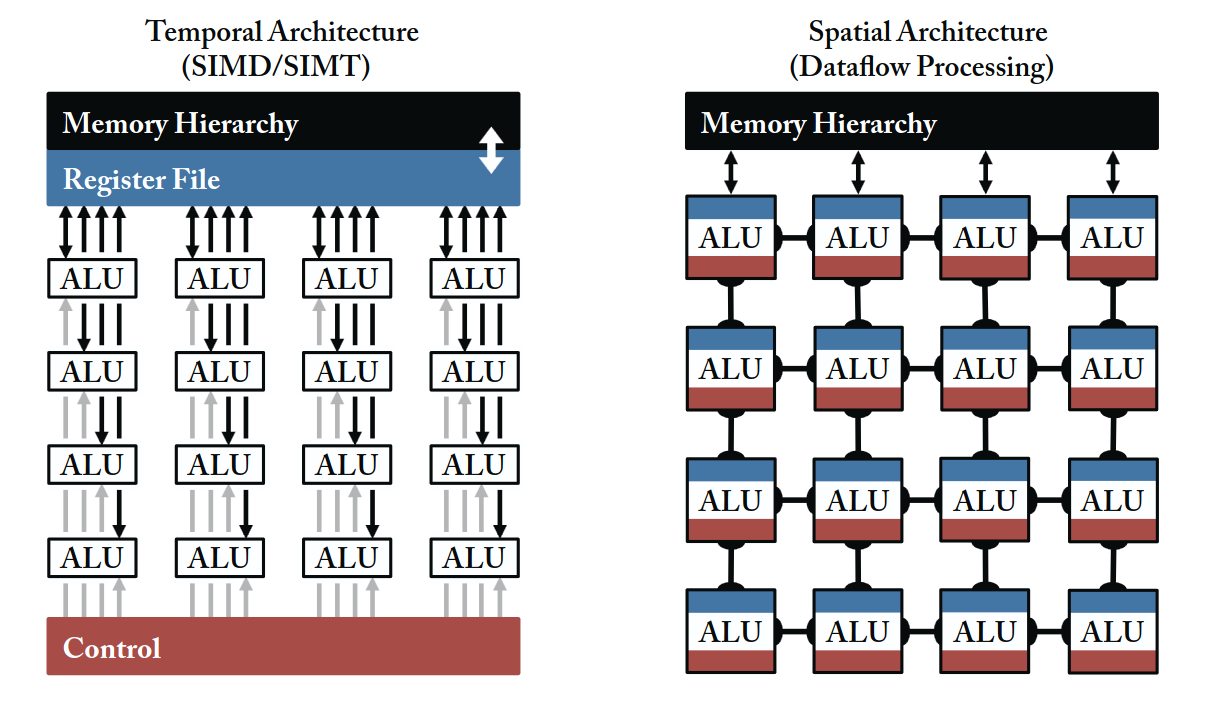
\includegraphics[width=\textwidth]{dnns-4.1.png}
                \caption{Temporal vs. Spatial Architecture}
            \end{figure}
        \end{column}
    \end{columns}
\end{frame}
\begin{frame}{Dataflows \& NoC Connectivity}
    \begin{columns}[c]
        \begin{column}{0.65\textwidth}
        \begin{itemize}
            \item \textbf{Dataflow Taxonomy}: Loop-nest ordering prioritizes stationarity (\textit{WS}, \textit{OS}, \textit{IS}, or \textit{RS}) to minimize memory access energy.
            \item \textbf{NoC Connectivity}: Trade-off between hardware bandwidth cost and spatial data reuse capability.
        \end{itemize}
        \begin{figure}
            \centering
            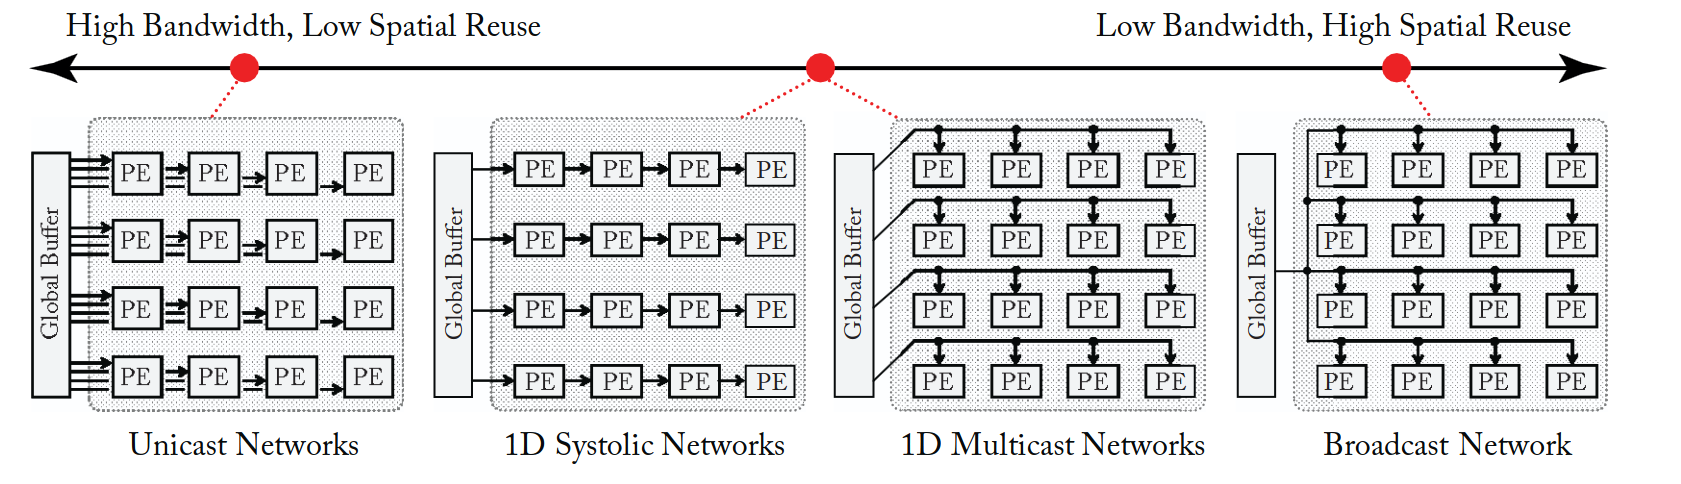
\includegraphics[width=1\textwidth]{dnns-5.32.png}
            \caption{NoC Topologies: Bandwidth vs. Spatial Reuse Trade-off}
        \end{figure}
        \end{column}

        \begin{column}{0.4\textwidth}
            \begin{figure}
                \centering
                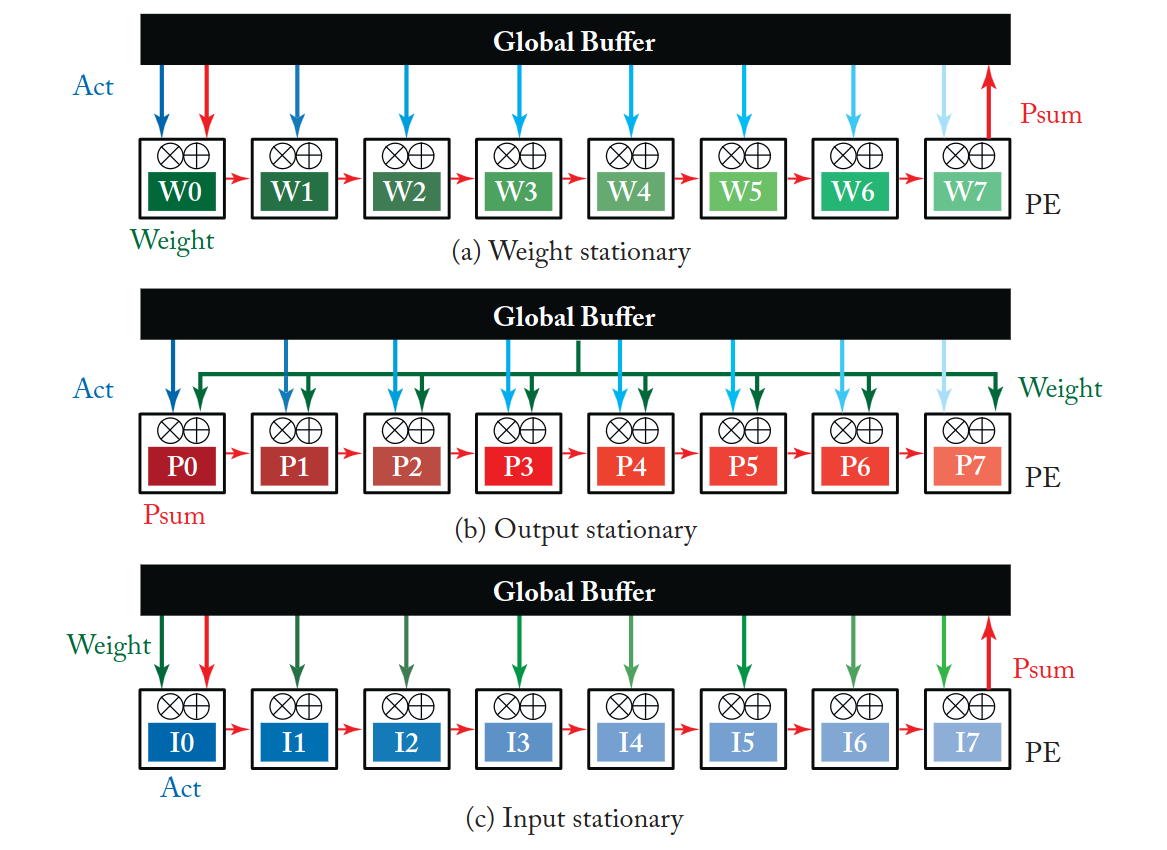
\includegraphics[width=1.1\textwidth]{dnns-5.15.png}
                \caption{Datalow architectures}
            \end{figure}
        \end{column}
    \end{columns}
\end{frame}


\end{document}
